%% Requires compilation with XeLaTeX or LuaLaTeX
\documentclass[compress,10pt,xcolor={table,dvipsnames},t]{beamer}
\usetheme{diapo}
\usepackage{amsmath}
\DeclareMathOperator*{\argmax}{arg\,max}
\DeclareMathOperator*{\argmin}{argmin}
\usepackage{amssymb}
\usepackage{xcolor}
\usepackage[bottom]{footmisc}
\usepackage{multirow}
\usepackage{setspace}
\usepackage{caption}
\usepackage{array,multirow,makecell}
\usepackage{pifont}
\usepackage{tikz}
\usepackage{paralist}
\usepackage{appendixnumberbeamer}
%\usepackage[style=authoryear,sorting=nyt,doi=false,url=false,maxbibnames=99,date=year]{biblatex}
\usepackage[square]{natbib}
\bibliographystyle{plainnat}
\usepackage{etoolbox}
% box colorée dans équation
\usepackage[most]{tcolorbox}
\usepackage{tikz}
\usepackage{soul}
% pour l'indicatrice
\usepackage{dsfont}
\usepackage{cancel}
\usepackage{booktabs}
\usepackage{bm}

\setcellgapes{1pt}
\setlength{\parindent}{0pt}
\makegapedcells
\newcolumntype{R}[1]{>{\raggedleft\arraybackslash }b{#1}}
\newcolumntype{L}[1]{>{\raggedright\arraybackslash }b{#1}}
\newcolumntype{C}[1]{>{\centering\arraybackslash }b{#1}}
\renewcommand*{\bibfont}{\scriptsize}
\useoutertheme[subsection=false]{miniframes}
\makeatletter
%\patchcmd{\slideentry}{\advance\beamer@xpos by1\relax}{}{}{}
\def\beamer@subsectionentry#1#2#3#4#5{\advance\beamer@xpos by1\relax}%
\makeatother
\setbeamercolor*{mini frame}{fg=bulles,bg=bulles}
\hypersetup{
	colorlinks=true,
	urlcolor=blue,
	citecolor=other,
	linkcolor=title,
}

\title[PhiFEM]{Combining Finite Element Methods and Neural Networks to Solve Elliptic Problems on 2D Geometries}
% \subtitle{1st CSI}

\author{%
	Hélène Barucq\inst{1}, 
    Michel Duprez\inst{2}, 
    Florian Faucher\inst{1}, 
    Emmanuel Franck\inst{3}, 
    \textbf{Frédérique Lecourtier}\inst{2}, 
    Vanessa Lleras\inst{4},
    Victor Michel-Dansac\inst{3} and
    Nicolas Victorion\inst{1}
}

\institute{%
	\inst{1} Project-Team Makutu, Inria, TotalEnergies, Pau, France \\
	\inst{2} Project-Team MIMESIS, Inria, Strasbourg, France \\
    \inst{3} Project-Team MACARON, Inria, Strasbourg, France \\
    \inst{4} IMAG, University of Montpellier, Montpellier, France
}

\date{February 20, 2025}

\allowbreak

% u_chapeau (chapeau en couleur)
\usepackage{accents}
\newcommand{\uchapeau}[1]{\accentset{\textcolor{red}{\wedge}}{#1}}
\newcommand{\refappendix}[1]{\tikz[baseline=(char.base)]{\node[framednumber] (char) {\hyperlink{#1}{\small \textcolor{white}{Appendix \ref*{#1}}}};}}

\tikzset{
	framednumber/.style={
		draw=appendix,% Couleur de la bordure
		fill=appendix, % Couleur de fond
		rounded corners, % Coins arrondis
		inner sep=2pt,  % Espace intérieur
	}
}

% numérotation et label des appendix
\newcounter{appendixframenumber}
\setcounter{appendixframenumber}{1}

\makeatletter
\newcommand{\labelappendixframe}[1]{%
	\protected@write\@auxout{}{%
		\string\newlabel{#1}{{\theappendixframenumber}{\thepage}}%
	}%
	\hypertarget{#1}{}
}	
\makeatother

% barre en couleur terme dans équation
\newcommand\Ccancel[2][black]{\renewcommand\CancelColor{\color{#1}}\cancel{#2}}

% chifrre romain dans le texte
\makeatletter
\newcommand*{\rom}[1]{\expandafter\@slowromancap\romannumeral #1@}
\makeatother

% warning
\newcommand{\warning}{{\fontencoding{U}\fontfamily{futs}\selectfont\char 49\relax}}

\newcommand{\insertsectionheadSubtitle}{}

\newtcbtheorem{mytheo}{Theorem}{colback=other, % Couleur de fond de la boîte
	colframe=other, % Couleur du cadre de la boîte
	arc=2mm, % Rayon de l'arrondi des coins
	boxrule=0.5pt, % Épaisseur du cadre de la boîte
	breakable, enhanced jigsaw,
	width=\linewidth,
	opacityback=0.1
	}{th}

\newcommand*{\footcite}[1]{\footnote[frame,1]{\citep{#1}}}

\usepackage{amssymb}
\usepackage{mathtools}
\usepackage{pgfplots}
\usepackage{pgfplotstable}
% \usepackage{filecontents}
\usepackage{datatool}
\usepackage{fp}
\usetikzlibrary{backgrounds}

\pgfplotsset{
    compat=newest,
}
\pgfplotsset{
    smaller labels/.style={
        label style={font=\footnotesize},
        tick label style={font=\footnotesize}
    }
}
\tikzset{font=\small}
\usetikzlibrary{
    fpu,
    fixedpointarithmetic,
    babel,
    external,
    arrows.meta,
    plotmarks,
    positioning,
    angles,
    quotes,
    intersections,
    calc,
    spy,
    decorations.pathreplacing,
    matrix,
    fit,
}
\usepgfplotslibrary{fillbetween}

% Define colors
\definecolor{femcolor}{RGB}{51, 138, 55} %Green (27,158,119)
\definecolor{addcolor}{RGB}{217,95,2} %Orange
\definecolor{addsobcolor}{RGB}{199,39,34} %Red (sob or other)
\definecolor{multcolor3}{RGB}{117,112,179} %Purple 
\definecolor{multcolor100}{RGB}{0,0,0} %Black (+ empty marker)
\definecolor{multcolor0weak}{RGB}{49, 73, 181} %Blue
\definecolor{multcolor0strong}{RGB}{49, 181, 161} %Cyan

% Define line styles according to the method 
% FEM : solid
% Add : dashed
% Mult : dotted

% Define marker styles according to the degree
% P1 : square
% P2 : circle
% P3 : triangle

%________________ error lines (by Ricardo Costa) ________________

% argument 1: slopes (e.g. {4,6})
% argument 2: x position of the bottom left corner
% argument 3: y position of the bottom left corner
% argument 4: x length

\makeatletter

\newcommand{\printslopeinv}[4]{
    \tikzset{fixed point arithmetic}
    % get arguments
    \def\nero@printslope@orderlist{#1}
    \edef\nero@printslope@xpos{#2}
    \edef\nero@printslope@ypos{#3}
    \edef\nero@printslope@width{#4}
    % get points position
    \pgfmathparse{\nero@printslope@xpos+\nero@printslope@width}
    \edef\nero@printslope@px{\pgfmathresult}
    \edef\nero@printslope@py{\nero@printslope@ypos}
    \edef\nero@printslope@qx{\pgfmathresult}
    \edef\nero@printslope@ry{\nero@printslope@ypos}
    \foreach \nero@printslope@order in {#1}{
        \pgfmathparse{
        ((\nero@printslope@px/\nero@printslope@xpos)^(\nero@printslope@order))*\nero@printslope@ypos}
        \edef\nero@printslope@qy{\pgfmathresult}
            \edef\nero@aux1{\noexpand\draw[line width=0.6pt]
            (axis cs:\nero@printslope@xpos,\nero@printslope@ypos)
            -- (axis cs:\nero@printslope@qx,\nero@printslope@qy)
            -- (axis cs:\nero@printslope@px,\nero@printslope@py);}
        \nero@aux1
        % slope label
        \pgfmathparse{10^((ln(\nero@printslope@ry)+ln(\nero@printslope@qy))/(ln(10)*2))}
        \edef\nero@printslope@labelpos{\pgfmathresult}
        \edef\nero@aux2{\noexpand\node[anchor=west] at
            (axis cs:\nero@printslope@qx,\nero@printslope@labelpos)
            {\noexpand\tiny \nero@printslope@order};}
        \nero@aux2
        \global\edef\nero@printslope@ry{\nero@printslope@qy}
    }
    % base line
    \draw[line width=0.6pt] (axis cs:\nero@printslope@xpos,\nero@printslope@ypos)
        |- (axis cs:\nero@printslope@px,\nero@printslope@py);
    % label of base line
    \pgfmathparse{10^((ln(\nero@printslope@px)+ln(\nero@printslope@xpos))/(ln(10)*2))}
    \edef\nero@printslope@labelpos{\pgfmathresult}
    \node[anchor=north] at (axis cs:\nero@printslope@labelpos,\nero@printslope@ypos) {\tiny 1};
}

\makeatother

\newlength{\plotwidth}
\setlength{\plotwidth}{0.54\textwidth}
\newlength{\plotheight}
\setlength{\plotheight}{0.4\textwidth}

\gdef\iterator{0}

\newenvironment{cvgh}[4]{
    \begin{tikzpicture}
        \edef\filename{#1}
        \edef\legendcolumns{#2}
        \edef\slopes{#3}
        \edef\ypos{#4}

        % Read the CSV file into a table
        \pgfplotstableread[col sep=comma]{\filename}\datatable

        % Obtenir le second élément
        \pgfmathtruncatemacro{\secondrow}{1} % Index de la dernière ligne
        \pgfplotstablegetelem{\secondrow}{h}\of\datatable
        \pgfmathsetmacro{\second}{\pgfplotsretval} % Dernière valeur de h_rounded

        % Obtenir le premier élément
        \pgfmathtruncatemacro{\firstrow}{0} % Index de l'avant-dernière ligne
        \pgfplotstablegetelem{\firstrow}{h}\of\datatable
        \pgfmathsetmacro{\first}{\pgfplotsretval} % Avant-dernière valeur de h_rounded

        % Calculer la différence entre les deux
        \pgfmathsetmacro{\diff}{\first - \second}

        %update iterator
        \pgfmathtruncatemacro{\iterator}{\iterator+1}

        \begin{loglogaxis}[
            smaller labels,
            name = left_plot,
            % axis lines
            axis lines = left,
            enlarge x limits={abs=10pt},
            enlarge y limits={abs=10pt},
            % axis x line shift = -5pt,
            axis y line shift = -5pt,
            % labels
			xmode=log,
            xlabel = {$h$},
            ylabel = {\rotatebox{270}{$L^2$}},
            xlabel style={at={(ticklabel* cs:1.01)},anchor=west},
            ylabel style={at={(ticklabel* cs:1.01)},anchor=west},
            % ticks and labels
            xtick=data,
            xticklabels from table={\datatable}{h},
            width=\plotwidth, height=\plotheight,
            mark options={solid, scale=1},
            grid = major,
            legend columns=\legendcolumns,
            legend to name=leg:legendFEMCORR_\iterator,
            legend image post style={mark options={solid, scale=1},xscale=0.8},
        ]
        \expandafter\printslopeinv\expandafter{\slopes}{\second}{\ypos}{\diff}
    }
    {
        \end{loglogaxis}
        \node[yshift=-20pt] at (left_plot.outer south) {\pgfplotslegendfromname{leg:legendFEMCORR_\iterator}};

    \end{tikzpicture}
}

\newenvironment{cvghline}[4]{
    \begin{tikzpicture}
        \edef\filename{#1}
        \edef\legendcolumns{#2}
        \edef\slopes{#3}
        \edef\ypos{#4}

        % Read the CSV file into a table
        \pgfplotstableread[col sep=comma]{\filename}\datatable

        % Obtenir le second élément
        \pgfmathtruncatemacro{\secondrow}{1} % Index de la dernière ligne
        \pgfplotstablegetelem{\secondrow}{h}\of\datatable
        \pgfmathsetmacro{\second}{\pgfplotsretval} % Dernière valeur de h_rounded

        % Obtenir le premier élément
        \pgfmathtruncatemacro{\firstrow}{0} % Index de l'avant-dernière ligne
        \pgfplotstablegetelem{\firstrow}{h}\of\datatable
        \pgfmathsetmacro{\first}{\pgfplotsretval} % Avant-dernière valeur de h_rounded

        % Calculer la différence entre les deux
        \pgfmathsetmacro{\diff}{\first - \second}

        %update iterator
        \pgfmathtruncatemacro{\iterator}{\iterator+1}

        \begin{loglogaxis}[
            smaller labels,
            name = left_plot,
            % axis lines
            axis lines = left,
            enlarge x limits={abs=10pt},
            enlarge y limits={abs=10pt},
            % axis x line shift = -5pt,
            axis y line shift = -5pt,
            % labels
			xmode=log,
            xlabel = {$h$},
            ylabel = {\rotatebox{270}{$L^2$}},
            xlabel style={at={(ticklabel* cs:1.01)},anchor=west},
            ylabel style={at={(ticklabel* cs:1.01)},anchor=west},
            % ticks and labels
            xtick=data,
            xticklabels from table={\datatable}{h},
            width=\plotwidth, height=\plotheight,
            mark options={solid, scale=1},
            grid = major,
            legend columns=\legendcolumns,
            legend to name=leg:legendFEMCORR_\iterator,
            legend image post style={mark options={solid, scale=1},xscale=0.8},
        ]
        \expandafter\printslopeinv\expandafter{\slopes}{\second}{\ypos}{\diff}
    }
    {
        \end{loglogaxis}
        \node[yshift=-20pt] at (left_plot.outer south) {\pgfplotslegendfromname{leg:legendFEMCORR_\iterator}};
        
        \draw[black, line width=0.4mm] (0.1,1.9) -- (4.7,1.9) node[anchor=west, xshift=2pt] {$e$};

    \end{tikzpicture}
}

\newcommand{\cvgFEMCorrAlldeg}[3]{
    \edef\fem{#1}
    \edef\add{#2}

    \begin{cvgh}{\fem}{3}{2,3,4}{#3}
        % Complete the legend
        \addlegendentry{\,FEM $\mathbb{P}_1$\;}
        \addlegendentry{\,FEM $\mathbb{P}_2$\;}
        \addlegendentry{\,FEM $\mathbb{P}_3$\;}
        \addlegendentry{\,Add $\mathbb{P}_1$\;}
        \addlegendentry{\,Add $\mathbb{P}_2$\;}
        \addlegendentry{\,Add $\mathbb{P}_3$\;}

        % Plot FEM
        \addplot [style={solid}, mark=square*, mark size=2, color=femcolor, line width=0.8pt ]
        table [x=h, y=P1, col sep=comma]
            {\fem};
        
        \addplot [style={solid}, mark=*, mark size=2, color=femcolor, line width=0.8pt ]
        table [x=h, y=P2, col sep=comma]
            {\fem};
        
        \addplot [style={solid}, mark=triangle*, mark size=2, color=femcolor, line width=0.8pt ]
        table [x=h, y=P3, col sep=comma]
            {\fem};

        % Plot Add
        \addplot [style={dashed}, mark=square*, mark size=2, color=addcolor, line width=0.8pt ]
        table [x=h, y=P1, col sep=comma]
            {\add};

        \addplot [style={dashed}, mark=*, mark size=2, color=addcolor, line width=0.8pt ]
        table [x=h, y=P2, col sep=comma]
            {\add};

        \addplot [style={dashed}, mark=triangle*, mark size=2, color=addcolor, line width=0.8pt ]
        table [x=h, y=P3, col sep=comma]
            {\add};

    \end{cvgh}
}

\newcommand{\cvgFEMCorrAlldegLine}[3]{
    \edef\fem{#1}
    \edef\add{#2}

    \begin{cvghline}{\fem}{3}{2,3,4}{#3}
        % Complete the legend
        \addlegendentry{\,FEM $\mathbb{P}_1$\;}
        \addlegendentry{\,FEM $\mathbb{P}_2$\;}
        \addlegendentry{\,FEM $\mathbb{P}_3$\;}
        \addlegendentry{\,Add $\mathbb{P}_1$\;}
        \addlegendentry{\,Add $\mathbb{P}_2$\;}
        \addlegendentry{\,Add $\mathbb{P}_3$\;}

        % Plot FEM
        \addplot [style={solid}, mark=square*, mark size=2, color=femcolor, line width=0.8pt ]
        table [x=h, y=P1, col sep=comma]
            {\fem};
        
        \addplot [style={solid}, mark=*, mark size=2, color=femcolor, line width=0.8pt ]
        table [x=h, y=P2, col sep=comma]
            {\fem};
        
        \addplot [style={solid}, mark=triangle*, mark size=2, color=femcolor, line width=0.8pt ]
        table [x=h, y=P3, col sep=comma]
            {\fem};

        % Plot Add
        \addplot [style={dashed}, mark=square*, mark size=2, color=addcolor, line width=0.8pt ]
        table [x=h, y=P1, col sep=comma]
            {\add};

        \addplot [style={dashed}, mark=*, mark size=2, color=addcolor, line width=0.8pt ]
        table [x=h, y=P2, col sep=comma]
            {\add};

        \addplot [style={dashed}, mark=triangle*, mark size=2, color=addcolor, line width=0.8pt ]
        table [x=h, y=P3, col sep=comma]
            {\add};

    \end{cvghline}
}

\newcommand{\cvgFEMCorrMultOnedeg}[6]{
    \edef\fem{#1}
    \edef\femsec{#2}
    \edef\add{#3}
    \edef\mult{#4}
    \edef\multHundred{#5}

    \begin{cvgh}{\fem}{3}{2,3}{#6}
        % Complete the legend
        \addlegendentry{\,FEM $\mathbb{P}_1$\;}
        \addlegendentry{\,Mult $\mathbb{P}_1$ (M=3)\;}
        \addlegendentry{\,Add $\mathbb{P}_1$\;}
        \addlegendentry{\,FEM $\mathbb{P}_2$\;}
        \addlegendentry{\,Mult $\mathbb{P}_1$ (M=100)\;}

        % Plot the data
        \addplot [style={solid}, mark=square*, mark size=2, color=femcolor, line width=0.8pt ]
        table [x=h, y=err, col sep=comma]
            {\fem};

        \addplot [style={dotted}, mark=square*, mark size=2, color=multcolor3, line width=1.0pt ]
        table [x=h, y=err, col sep=comma]
            {\mult};

        \addplot [style={dashed}, mark=square*, mark size=2, color=addcolor, line width=0.8pt ]
        table [x=h, y=err, col sep=comma]
            {\add};

        \addplot [style={solid}, mark=*, mark size=2, color=femcolor, line width=0.8pt ]
        table [x=h, y=err, col sep=comma]
            {\femsec};

        \addplot [style={dotted}, mark=square, mark size=2, color=multcolor100, line width=1.0pt ]
        table [x=h, y=err, col sep=comma]
            {\multHundred};
    \end{cvgh}
}
\usepackage{booktabs}
\usepackage{xcolor}

% gains pour tous les q
\newcommand{\gainstableallq}[1]{
    \pgfplotstabletypeset[
        col sep=comma,
        every head row/.style={
        before row={\toprule[1.pt]
        & \multicolumn{3}{c}{\textbf{Gains in $L^2$ rel error}} \\
		& \multicolumn{3}{c}{\textbf{of our method w.r.t. FEM}} \\
		\cmidrule(lr){2-4}
        },
        after row=\cmidrule(lr){1-1} \cmidrule(lr){2-4}},
        every last row/.style={after row=\bottomrule[1.pt]},
        every nth row={1}{before row=\cmidrule(lr){1-1} \cmidrule(lr){2-4}},
		columns/q/.style={column name=\textbf{k}},
        columns/min_FEM/.style={column name=\textbf{min},fixed},
        columns/max_FEM/.style={column name=\textbf{max},fixed},
        columns/mean_FEM/.style={column name=\textbf{mean},fixed,
            postproc cell content/.append style={
                /pgfplots/table/@cell content/.add={\color{red}}{},
            }
        },
        columns={q,min_FEM,max_FEM,mean_FEM},
        precision=2
    ]{#1}
}


\usepackage{booktabs}

% costs pour tous les q : N et DoFs
\newcommand{\coststableallq}[1]{
    \pgfplotstabletypeset[
        col sep=comma,
        every head row/.style={
        before row={\toprule[1.pt]
        & & \multicolumn{2}{c}{\textbf{$N_\text{dofs}$}} \\
		\cmidrule(lr){3-4}
        },
        after row=\cmidrule(lr){1-1} \cmidrule(lr){2-2} \cmidrule(lr){3-4}},
        every last row/.style={after row=\bottomrule[1.pt]},
        every nth row={2}{before row=\cmidrule(lr){1-1} \cmidrule(lr){2-2} \cmidrule(lr){3-4}},
		columns/q/.style={column name=\textbf{k}},
        columns/e/.style={column name=\textbf{e},sci},
		columns/FEM_dofs/.style={column name=\textbf{FEM},fixed},
        columns/Add_dofs/.style={column name=\textbf{Add},fixed},
        columns={q,e,FEM_dofs,Add_dofs},
        precision=2
    ]{#1}
}

\begin{document}
	\nocite{*}
	
	\renewcommand{\inserttotalframenumber}{\pageref{lastslide}}
	
	{\setbeamertemplate{footline}{} 
		\BackgroundTitle	
		\begin{frame}
			\maketitle
		\end{frame}
	}
	\addtocounter{framenumber}{-1} 	
	
	\AtBeginSection[]{
		{\setbeamertemplate{footline}{}
			\begin{frame}
				\vfill
				\centering
				\begin{beamercolorbox}[sep=5pt,shadow=true,rounded=true]{subtitle}
					\usebeamerfont{title}\insertsectionhead\par%
					\vspace{0.5cm} % Ajustez l'espacement selon vos besoins
					\usebeamerfont{classic}\usebeamercolor[fg]{classic}\insertsectionheadSubtitle
				\end{beamercolorbox}
				%\tableofcontents[sectionstyle=hide,subsectionstyle=show]
				
				%subsectionstyle=⟨style for current subsection⟩/⟨style for other subsections in current section⟩/⟨style for subsections in other sections⟩
				\tableofcontents[sectionstyle=hide,subsectionstyle=show/show/hide]
				\vfill
			\end{frame}
		}
		\addtocounter{framenumber}{-1} 
	}
	
	\AtBeginSubsection[]{
		{\setbeamertemplate{footline}{}
			\begin{frame}
				\vfill
				\centering
				\begin{beamercolorbox}[sep=5pt,shadow=true,rounded=true]{subtitle}
					\usebeamerfont{title}\insertsectionhead\par%
					\vspace{0.5cm} 
				\end{beamercolorbox}
				\tableofcontents[sectionstyle=hide,subsectionstyle=show/shaded/hide]
				\vfill
			\end{frame}
		}
		\addtocounter{framenumber}{-1} 
	}
	
	\Background
	\section*{Introduction}
	\begin{frame}{Scientific context}
    \textbf{Context :} Create real-time digital twins of an organ (such as the liver).

    \textbf{$\phi$-FEM Method :} New fictitious domain finite element method.

    \begin{enumerate}[\ding{217}]
        \item domain given by a level-set function $\Rightarrow$ don't require a mesh fitting the boundary 
        \item allow to work on complex geometries 
        \item ensure geometric quality 
        % \item Cartesian grid adapted for neural networks
    \end{enumerate}
    
    \begin{center}
        \pgfimage[width=0.65\linewidth]{images/intro/context_geometry.png}
    \end{center}	

    \textit{Practical case:} Real-time simulation, shape optimization...
\end{frame}

\begin{frame}{Objective}
    \textbf{Current Objective :} Develop hybrid finite element / neural network methods.

	\begin{center}
		\begin{tcolorbox}[
			colback=white, % Couleur de fond de la boîte
			colframe=other, % Couleur du cadre de la boîte
			arc=2mm, % Rayon de l'arrondi des coins
			boxrule=0.5pt, % Épaisseur du cadre de la boîte
			breakable, enhanced jigsaw,
			width=0.8\linewidth
			]
			
			\textbf{OFFLINE :}
			
			\begin{figure}[htb]
				\centering
				\resizebox{\textwidth}{!}{%
					\begin{tikzpicture}
						\node at (0,0.8) {Several Geometries};
						\node[draw=none, inner sep=0pt] at (0,0) {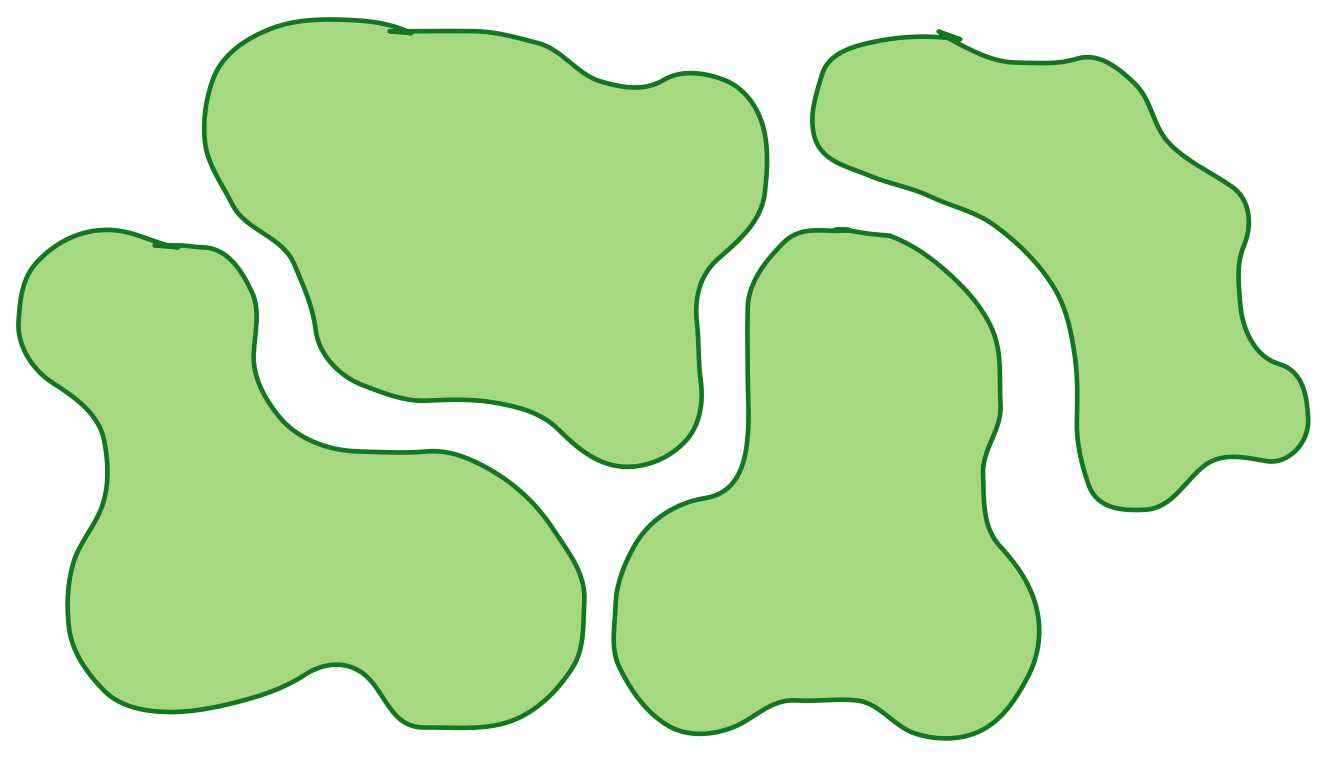
\includegraphics[width=2cm]{images/intro/objective_geom.png}};
						\node[title,font=\Large] at (1.6,0.1) {+};
						\node at (3.5,0.8) {Several Functions};
						\node[draw=none, inner sep=0pt] at (3.5,0) {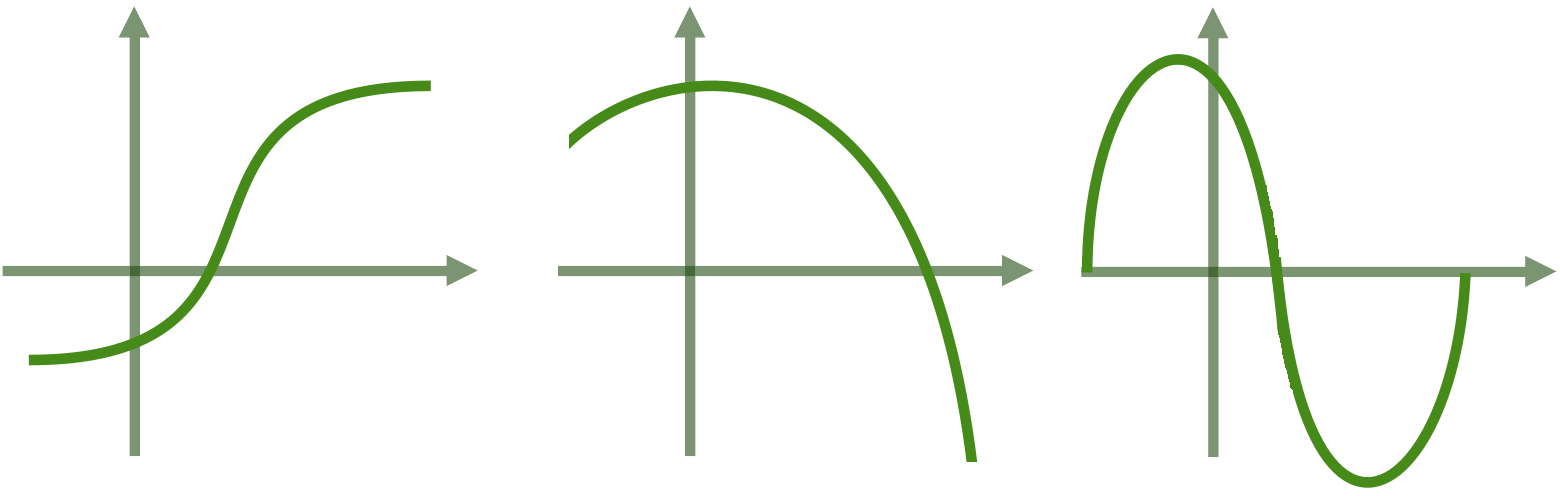
\includegraphics[width=3cm]{images/intro/objective_fct.png}};
						
						% Ajouter une flèche entre les deux rectangles
						\draw[->, title, line width=1.5pt] (5.5,0.1) -- (6.5,0.1);
						%		
						\node at (8,0.8) {Train a PINNs};
						\node[draw=none, inner sep=0pt] at (8,-0.1) {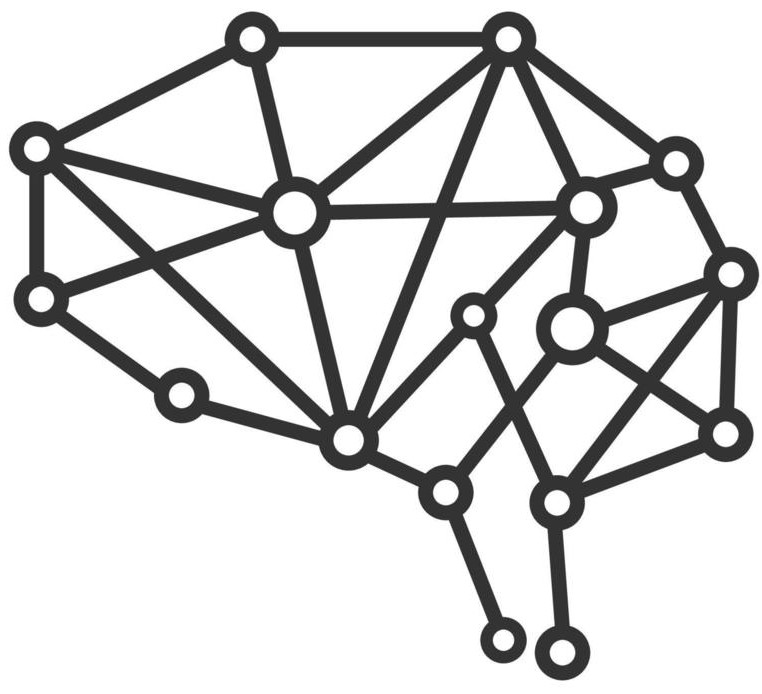
\includegraphics[width=1.5cm]{images/intro/objective_pinns.jpg}};				
					\end{tikzpicture}
				}%
			\end{figure}
			
			\textbf{ONLINE :}
			
			\vspace{-25pt}
			
			\begin{figure}[htb]
				\centering
				\resizebox{\textwidth}{!}{%
					\begin{tikzpicture}
						\node at (0,0.8) {1 Geometry - 1 Function};
						\node[draw=none, inner sep=0pt] at (0,0) {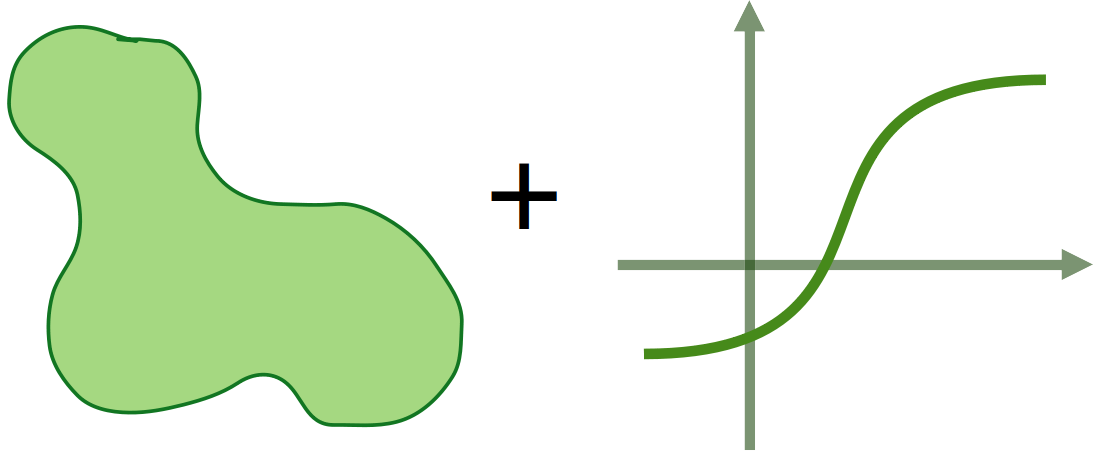
\includegraphics[width=2cm]{images/intro/objective_onegeom_onefct.png}};
						%		\node[title,font=\Large] at (1.6,0.1) {+};
						%		\node at (3.5,0.8) {Several Functions};
						%		\node[draw=none, inner sep=0pt] at (3.5,0) {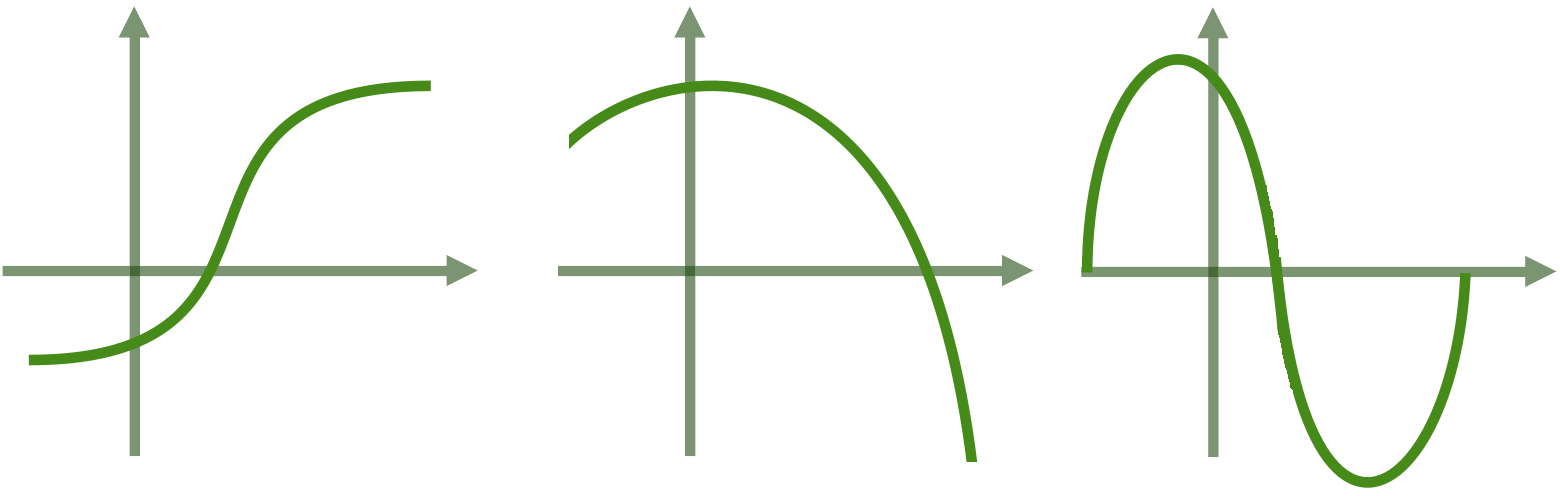
\includegraphics[width=3cm]{images/intro/objective_fct.png}};
						
						\draw[->, title, line width=1.5pt] (2,0.1) -- (3,0.1);
						
						\node[align=center] at (4,1) {Get PINNs \\ prediction};
						\node[draw=none, inner sep=0pt] at (4,-0.1) {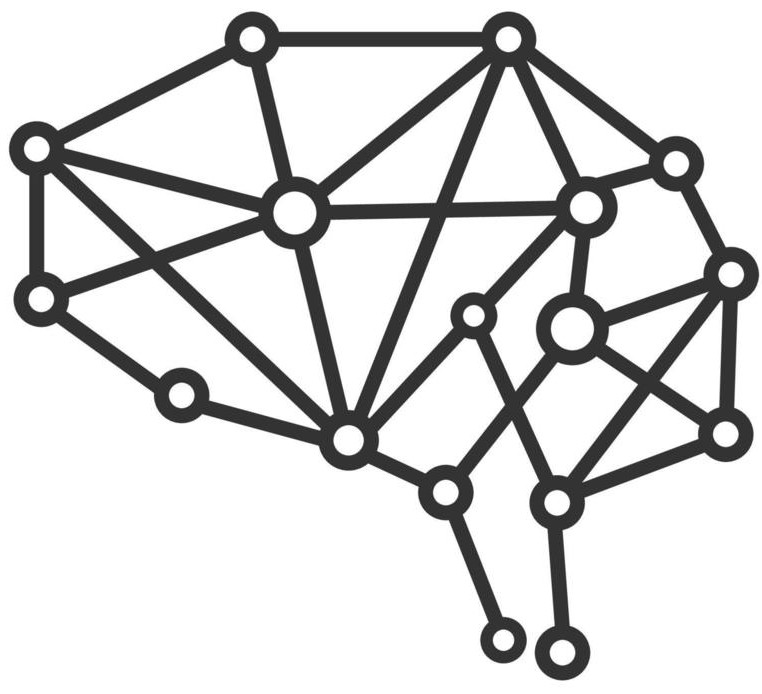
\includegraphics[width=1.5cm]{images/intro/objective_pinns.jpg}};
						
						% Ajouter une flèche entre les deux rectangles
						\draw[->, title, line width=1.5pt] (5.5,0.1) -- (6.5,0.1);
						%		
						\node[align=center] at (8,1) {Correct prediction \\ with $\phi$-FEM};
						\node[draw=none, inner sep=0pt] at (8,-0.1) {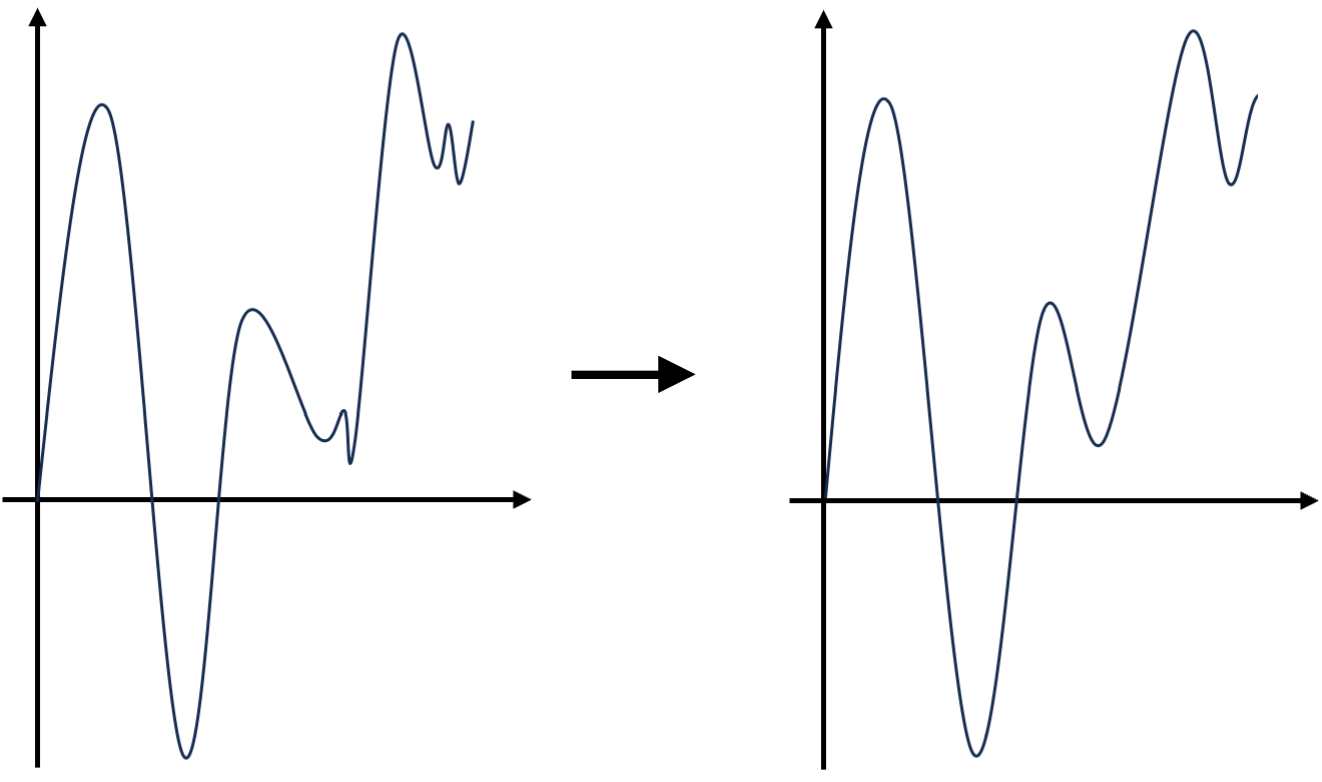
\includegraphics[width=2.5cm]{images/intro/objective_corr.png}};		
					\end{tikzpicture}
				}%
			\end{figure}
		\end{tcolorbox}
	\end{center}

    \textbf{Evolution :}

    \small
    % \setstretch{0.5}
    \begin{itemize}
        \item Geometry : 2D, simple, fixed (as circle, ellipse..) $ \; \rightarrow \;$ 3D / complex / variable
        \item PDE : simple, static (Poisson problem) $\; \rightarrow \;$ complex / dynamic (elasticity, hyper-elasticity)
        \item Neural Network : simple and defined everywhere (PINNs) $\; \rightarrow \;$ Neural Operator
    \end{itemize}
\end{frame}

\begin{frame}{Problem considered}
    \textbf{Elliptic problem with Dirichlet conditions :} \\
    Find $u : \Omega \rightarrow \mathbb{R}^d (d=1,2,3)$ such that
    \begin{equation}
    	\left\{\begin{aligned}
    		&L(u)=-\nabla \cdot (A(x) \nabla u(x)) + c(x)u(x) = f(x) \quad \text{in } \Omega, \\
    		&u(x) = g(x) \quad \text{on } \partial \Omega
    	\end{aligned}\right. \label{edp}
    \end{equation}
	with $A$ a definite positive coercivity condition and $c$ a scalar. We consider $\Delta$ the Laplace operator, $\Omega$ a smooth bounded open set and $\Gamma$ its boundary. 
    
    \textbf{Weak formulation :}
    \begin{equation*}
    	\text{Find } u\in V \text{ such that } a(u, v) = l (v) \forall v\in V
    \end{equation*}
    
    with
    \begin{align*}
    	a(u,v)&=\int_{\Omega} (A(x)\nabla u(x)) \cdot \nabla v(x) + c(x)u(x)v(x) \, dx \\
    	l(v)&=\int_{\Omega} f(x)v(x) \, dx
    \end{align*}
    
    \footnotesize
    \textit{Remark :} For simplicity, we will not consider 1st order terms. 

%    We will define by
%    \begin{equation*}
%        ||u_{ex}-u_{method}||_{0,\Omega}^{(rel)}=\frac{\int_\Omega (u_{ex}-u_{method})^2}{\int_\Omega u_{ex}^2}
%    \end{equation*}
%    the relative error between
%    \begin{itemize}
%        \item $u_{ex}$ : the exact solution  
%        \item $u_{method}$ : the solution obtained by a method \\
%        (can be : FEM or $\phi$-FEM, a correction solver or the prediction of an neural network).
%    \end{itemize}
\end{frame}

\begin{frame}{Numerical methods}
	\textbf{Objective :} Show that the philosophy behind most ofd the methods are the same.
	\begin{center}
		Mesh-based methods \hspace{5pt} // \hspace{5pt} Physically informed learning
	\end{center}
	
	\textbf{Numerical methods :} Discrete an infinite-dimensional problem (unknown = function) and solve it in a finite-dimensional space (unknown = vector).
	\begin{enumerate}[\textbullet]
		\item \textbf{Encoding :} we encode the problem in a finite-dimensional space
		\item \textbf{Approximation :} solve the problem in finite-dimensional space
		\item \textbf{Decoding :} bring the solution back into infinite dimensional space
	\end{enumerate}
	
	\begin{center}
		\begin{tabular}{|c|c|c|}
			\hline
			\textbf{Encoding} & \textbf{Approximation} & \textbf{Decoding} \\
			\hline
			$f \; \rightarrow \theta_f$ & $\theta_f \; \rightarrow \theta_u$ & $\theta_u \; \rightarrow u_\theta$ \\
			\hline
		\end{tabular}
	\end{center}
\end{frame}

	
	\section{How improve PINN prediction with FEM ?}
	\subsection{Additive approach}

\begin{frame}{Additive approach}
	\textbf{Variational Problem :} Let $u_{\theta} \in H^{k+1}(\Omega)\cap H^1_0(\Omega)$.
	
	\vspace{-5pt}
	\begin{equation}
		\label{eq:weakplus}
		\text{Find } p_h^+ \in V_h^0 \text{ such that}, \forall v_h \in V_h^0, a(p_h^+,v_h) = l(v_h) - a(u_{\theta},v_h),\tag{$\mathcal{P}_h^+$}
	\end{equation}
	
	\vspace{5pt}
	\begin{minipage}[t]{0.6\linewidth}
		with the \textcolor{red}{enriched trial space $V_h^+$} defined by
		\begin{equation*}
			V_h^+ = \left\{
			u_h^+= u_{\theta} + p_h^+, \quad p_h^+ \in V_h^0
			\right\}.
		\end{equation*}
	
		\vspace{20pt}
	
		\textbf{General Dirichlet BC :} If $u=g$ on $\partial \Omega$, then
		\[
			p_h^+ = g - u_{\theta} \text{\quad on } \partial \Omega,
		\]
		with $u_\theta$ the PINN prior. 
	\end{minipage} \qquad \begin{minipage}[t][][b]{0.28\linewidth}
		\vspace{-15pt}
		\centering
		\pgfimage[width=\linewidth]{images/correction/correction.pdf}
	\end{minipage}
\end{frame}

\begin{frame}{Convergence analysis}
	\vspace{-10pt}
	\hypersetup{
		citecolor=white,
	}

	\begin{mytheo}{Convergence analysis of the standard FEM \footnotesize\citep{Ern2004TheoryAP}\normalsize}{fem}
		We denote $u_h\in V_h$ the solution of \eqref{eq:weakform} with $V_h$ the standard trial space. Then,
		\vspace{-5pt}
		\begin{equation*}
			| u-u_h|_{H^1} \leqslant C_{H^1} \, h^{k} |u|_{H^{k+1}},
		\end{equation*}
		\begin{equation*}
			\| u-u_h\|_{L^2} \leqslant C_{L^2} \, h^{k+1} |u|_{H^{k+1}}.
		\end{equation*}
	\end{mytheo}
	
	\begin{mytheo}{Convergence analysis of the enriched FEM \footnotesize\citep{ours_2025}\normalsize}{add}
		We denote $u_h^+\in V_h^+$ the solution of \eqref{eq:weakplus} with $V_h^+$ the enriched trial space. Then,
		\vspace{-5pt}
		\begin{equation*}
			| u-u_h^+|_{H^1} \leqslant \fcolorbox{orange}{other!10!white}{$\frac{| u-u_{\theta} |_{H^{k+1}}}{| u |_{H^{k+1}}}$} \left(C_{H^1} \, h^{k} |u|_{H^{k+1}}\right),
		\end{equation*}
		\begin{equation*}
			\| u-u_h^+\|_{L^2} \leqslant \fcolorbox{orange}{other!10!white}{$\frac{| u-u_{\theta} |_{H^{k+1}}}{| u |_{H^{k+1}}}$} \left(C_{L^2} \, h^{k+1} |u|_{H^{k+1}}\right).
		\end{equation*}
	\end{mytheo}

	\hypersetup{
		citecolor=other,
	}

	\footnotesize
	\textcolor{orange}{Gains of the additive approach.}
\end{frame}

\subsection{Numerical results \filledstar}

\begin{frame}{1st problem considered} 
	\textbf{Problem statement:} Considering an \textcolor{red}{Anisotropic Elliptic problem with Dirichlet BC}:
	\vspace{-5pt}
	\begin{equation*}
		\left\{
		\begin{aligned}
			-\text{div}(D\nabla u) & = f, \; &  & \text{in } \; \Omega, \\
			u         & =0, \;  &  & \text{on } \; \partial\Omega,
		\end{aligned}
		\right.
		% \label{eq:Ell2D}\tag{$\mathcal{P}$}
	\end{equation*}

	with $\Omega=[0,1]^2$ and $\mathcal{M}=[0.4, 0.6]\times [0.4, 0.6]\times [0.01,1]\times [0.1,0.8]$ ($p=4$).
	
	\vspace{8pt}
	\textbf{Right-hand side :}

	\vspace{-5pt}
	\begin{equation*}
		f(\bm{x},\bm{\mu})=\exp\left(-\frac{(x-\mu_1)^2+(y-\mu_2)^2}{0.025\sigma^2}\right).
	\end{equation*}
	
	\textbf{Diffusion matrix :} (symmetric and positive definite)
	\begin{equation*}
		D(\bm{x},\bm{\mu})=\begin{pmatrix}
			\epsilon x^2+y^2 & (\epsilon-1)xy \\
			(\epsilon-1)xy & x^2+\epsilon y^2
		\end{pmatrix}.
	\end{equation*}

	\vspace{2pt}
	\small
	\textbf{PINN training:} Imposing BC exactly with a level-set function.
\end{frame}

\begin{frame}{Numerical results}
	\hspace{-5pt}\begin{minipage}[t]{0.46\linewidth}
		\textbf{Error estimates :} 1 set of parameters.
		$$\bm{\mu}^{(1)}=(0.51,0.54,0.52,0.55)$$
		\vspace{-35pt}
		\begin{figure}[H]
			\cvgFEMCorrAlldeg{images/numeric/elliptic/cvg/FEM_case3_v1_param1.csv}{images/numeric/elliptic/cvg/Corr_case3_v1_param1.csv}{1e-9}
		\end{figure}
	\end{minipage} \qquad \small
	\begin{minipage}[t]{0.48\linewidth}
	\end{minipage}
\end{frame}

\begin{frame}[noframenumbering]{Numerical results}
	\hspace{-5pt}\begin{minipage}[t]{0.46\linewidth}
		\textbf{Error estimates :} 1 set of parameters.
		$$\bm{\mu}^{(1)}=(0.51,0.54,0.52,0.55)$$
		\vspace{-35pt}
		\begin{figure}[H]
			\cvgFEMCorrAlldeg{images/numeric/elliptic/cvg/FEM_case3_v1_param1.csv}{images/numeric/elliptic/cvg/Corr_case3_v1_param1.csv}{1e-9}
		\end{figure}
	\end{minipage} \qquad \small
	\begin{minipage}[t]{0.48\linewidth}
		\textbf{Gains achieved :} $n_p=50$ sets of parameters.
		$$\mathcal{S}=\left\{\bm{\mu}^{(1)},\dots,\bm{\mu}^{(n_p)}\right\}$$
		\vspace{-15pt}
		\begin{table}[H]
			\gainstableallq{images/numeric/elliptic/gains/Tab_stats_case3_v1.csv}
		\end{table}

		\normalsize\centering\vspace{-20pt}
		$$N=20$$

		\vspace{-5pt}
		Gain : $\| u-u_h\|_{L^2} / \| u-u_h^+\|_{L^2}$ \\
		
		\small\vspace{8pt}
		Cartesian mesh : $N^2$ nodes.
	\end{minipage}
\end{frame}

\begin{frame}{Numerical solutions}
	\begin{figure}[!ht] \centering
		\includegraphics[width=0.33\linewidth]{images/numeric/elliptic/plots/standalone_solutions_cropped.pdf}		
		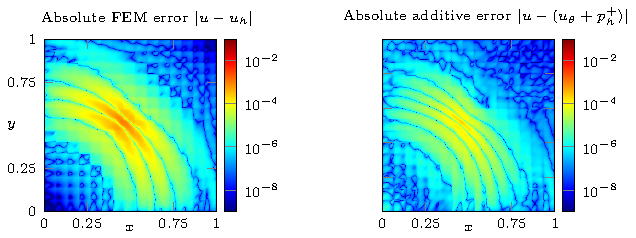
\includegraphics[width=0.7\linewidth]{images/numeric/elliptic/plots/standalone_errors.pdf}
	\end{figure}

	\vspace{-8pt}
	$$\bm{\mu}^{(2)}=(0.46,0.52,0.05,0.12)$$
\end{frame}

\begin{frame}{2nd problem considered} 
	\textbf{Problem statement:} Considering the \textcolor{red}{Poisson problem with mixed BC}:
	\vspace{-5pt}
	\begin{equation*}
		\left\{
		\begin{aligned}
			-\Delta u & = f, \; &  & \text{in } \; \Omega \times \mathcal{M}, \\
			u         & = g, \;  &  & \text{on } \; \Gamma_E \times \mathcal{M}, \\
			\smash{\frac{\partial u}{\partial n}}+u  & = g_R, \;  &  & \text{on } \; \Gamma_I \times \mathcal{M},
		\end{aligned}
		\right.
		% \label{eq:Lap2DMixed}\tag{$\mathcal{P}$}
	\end{equation*}

	with $\Omega=\{(x,y)\in\mathbb{R}^2, \; 0.25\le x^2+y^2\le 1\}$ and $\mathcal{M}=[2.4,2.6]$ ($p=1$).
		
	\vspace{8pt}
	\textbf{Analytical solution :}

	\vspace{-12pt}
	\begin{equation*}
		% \label{eq:analytical_solution_Lap2D}
		u(\bm{x};\bm{\mu})= 1 - \frac{\ln\big(\mu_1\sqrt{x^2+y^2}\big)}{\ln(4)},
	\end{equation*}
	\vspace{-5pt}
	
	\textbf{Boundary conditions :}
	\begin{equation*}
		g(\bm{x};\bm{\mu})=1 - \frac{\ln(\mu_1)}{\ln(4)} \quad \text{and} \quad g_R(\bm{x};\bm{\mu})=2 + \frac{4-\ln(\mu_1)}{\ln(4)}.
	\end{equation*}

	\vspace{2pt}
	\small
	\textbf{PINN training:} Imposing mixed BC exactly in the PINN\footcite{Sukumar_2022}.

	\vspace{8pt}
\end{frame}

\begin{frame}{Numerical results}
	\hspace{-5pt}\begin{minipage}[t]{0.46\linewidth}
		\textbf{Error estimates :} 1 set of parameters.
		$$\bm{\mu}^{(1)}=2.51$$
		\vspace{-35pt}
		\begin{figure}[H]
			\cvgFEMCorrAlldeg{images/numeric/poisson/mixed/cvg/FEM_case5_v2_param1.csv}{images/numeric/poisson/mixed/cvg/Corr_case5_v2_param1.csv}{1e-10}
		\end{figure}
	\end{minipage} \qquad \small
	\begin{minipage}[t]{0.48\linewidth}
		\textbf{Gains achieved :} $n_p=50$ sets of parameters.
		$$\mathcal{S}=\left\{\bm{\mu}^{(1)},\dots,\bm{\mu}^{(n_p)}\right\}$$
		\vspace{-15pt}
		\begin{table}[H]
			\gainstableallq{images/numeric/poisson/mixed/gains/Tab_stats_case5_v2.csv}
		\end{table}

		\normalsize\centering\vspace{-20pt}
		$$h=1.33\cdot 10^{-1}$$

		\vspace{-5pt}
		Gain : $\| u-u_h\|_{L^2} / \| u-u_h^+\|_{L^2}$ \\
		\end{minipage}
\end{frame}

\begin{frame}{Numerical solutions}
	\begin{figure}[!ht] \centering
		\includegraphics[width=0.31\linewidth]{images/numeric/poisson/mixed/plots/standalone_solutions_cropped.pdf}
		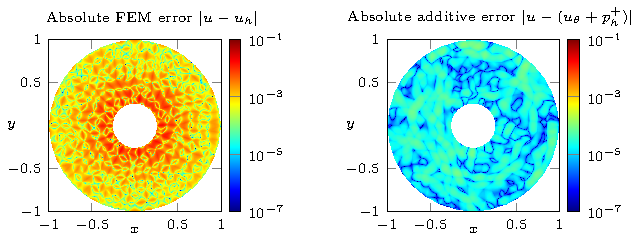
\includegraphics[width=0.7\linewidth]{images/numeric/poisson/mixed/plots/standalone_errors.pdf}
	\end{figure}

	\vspace{-8pt}
	$$\bm{\mu}^{(1)}=2.51 $$
\end{frame}

	\section{Numerical results}
	\subsection{2D Poisson problem on Square - Dirichlet BC}

\begin{frame}{Problem considered} 
	\textbf{Problem statement:} Consider the Poisson problem with Dirichlet BC:
	\vspace{-5pt}
	\begin{equation*}
		\left\{
		\begin{aligned}
			-\Delta u & = f, \; &  & \text{in } \; \Omega \times \mathcal{M}, \\
			u         & =0, \;  &  & \text{on } \; \partial\Omega \times \mathcal{M},
		\end{aligned}
		\right.
		% \label{eq:Lap2D}\tag{$\mathcal{P}$}
	\end{equation*}

	\vspace{-5pt}
	with $\Omega=[-0.5 \pi, 0.5 \pi]^2$ and $\mathcal{M}=[-0.5,0.5]^2$ ($p=2$ parameters).
		
	\vspace{8pt}
	\textbf{Analytical solution :}

	\vspace{-5pt}
	\begin{equation*}
		% \label{eq:analytical_solution_Lap2D}
		u(\bm{x},\bm{\mu})=\exp\left(-\frac{(x-\mu_1)^2+(y-\mu_2)^2}{2}\right)\sin(2 x)\sin(2 y).
	\end{equation*}

	\vspace{12pt}
	\textbf{PINN training:} MLP of 5 layers; LBFGs optimizer (5000 epochs). \\
	Imposing the Dirichlet BC exactly in the PINN with the levelset $\varphi$ defined by
	$$\varphi(\bm{x})=(x+0.5\pi)(x-0.5\pi)(y+0.5\pi)(y-0.5\pi).$$
	
	\small\vspace{4pt}
	Training time : less than 1 hour on a laptop GPU.
\end{frame}

\begin{frame}{Numerical results}
	\hspace{-5pt}\begin{minipage}[t]{0.46\linewidth}
		\textbf{Error estimates :} 1 set of parameters.
		$$\bm{\mu}^{(1)}=(0.05, 0.22) $$
		\vspace{-35pt}
		\begin{figure}[H]
			\cvgFEMCorrAlldeg{images/numeric/poisson/dirichlet/cvg/FEM_case1_v1_param1.csv}{images/numeric/poisson/dirichlet/cvg/Corr_case1_v1_param1.csv}{1e-10}
		\end{figure}
	\end{minipage} \qquad \small
	\begin{minipage}[t]{0.48\linewidth}
	\end{minipage}
\end{frame}

\begin{frame}[noframenumbering]{Numerical results}
	\hspace{-5pt}\begin{minipage}[t]{0.46\linewidth}
		\textbf{Error estimates :} 1  set of parameters.
		$$\bm{\mu}^{(1)}=(0.05, 0.22) $$
		\vspace{-35pt}
		\begin{figure}[H]
			\cvgFEMCorrAlldeg{images/numeric/poisson/dirichlet/cvg/FEM_case1_v1_param1.csv}{images/numeric/poisson/dirichlet/cvg/Corr_case1_v1_param1.csv}{1e-10}
		\end{figure}
	\end{minipage} \qquad \small
	\begin{minipage}[t]{0.48\linewidth}
		\textbf{Gains achieved :} $n_p=50$ sets of parameters.
		$$\mathcal{S}=\left\{\bm{\mu}^{(1)},\dots,\bm{\mu}^{(n_p)}\right\}$$
		\vspace{-15pt}
		\begin{table}[H]
			\gainstableallq{images/numeric/poisson/dirichlet/gains/Tab_stats_case1_v1.csv}
		\end{table}

		\normalsize\centering\vspace{-20pt}
		$$N=20$$

		\vspace{-5pt}
		Gain : $\| u-u_h\|_{L^2} / \| u-u_h^+\|_{L^2}$ \\
		
		\small\vspace{8pt}
		Cartesian mesh : $N^2$ nodes.
	\end{minipage}
\end{frame}

\begin{frame}[noframenumbering]{Numerical results}
	\hspace{-5pt}\begin{minipage}[t]{0.46\linewidth}
		\textbf{Error estimates :} 1 set of parameters.
		$$\bm{\mu}^{(1)}=(0.05, 0.22) $$
		\vspace{-35pt}
		\begin{figure}[H]
			\cvgFEMCorrAlldegLine{images/numeric/poisson/dirichlet/cvg/FEM_case1_v1_param1.csv}{images/numeric/poisson/dirichlet/cvg/Corr_case1_v1_param1.csv}{1e-10}
		\end{figure}
	\end{minipage} \qquad \small
	\begin{minipage}[t]{0.48\linewidth}
		\textbf{$N_\text{dofs}$ required to reach the same error $e$ :}

		\vspace{10pt}
		\begin{table}[H]
			\centering
			\coststableallq{images/numeric/poisson/dirichlet/costs/TabDoFs_case1_v1_param1.csv}
		\end{table}
	\end{minipage}
\end{frame}

\subsection{2D Anisotropic Elliptic problem on a Square - Dirichlet BC}

\begin{frame}{Problem considered} 
	\textbf{Problem statement:} Considering an Anisotropic Elliptic problem with Dirichlet BC:
	\vspace{-5pt}
	\begin{equation*}
		\left\{
		\begin{aligned}
			-\text{div}(D\nabla u) & = f, \; &  & \text{in } \; \Omega, \\
			u         & =0, \;  &  & \text{on } \; \partial\Omega,
		\end{aligned}
		\right.
		% \label{eq:Ell2D}\tag{$\mathcal{P}$}
	\end{equation*}

	with $\Omega=[0,1]^2$ and $\mathcal{M}=[0.4, 0.6]\times [0.4, 0.6]\times [0.01,1]\times [0.1,0.8]$ ($p=4$).
	
	\vspace{8pt}
	\textbf{Right-hand side :}

	\vspace{-5pt}
	\begin{equation*}
		f(\bm{x},\bm{\mu})=\exp\left(-\frac{(x-\mu_1)^2+(y-\mu_2)^2}{0.025\sigma^2}\right).
	\end{equation*}
	
	\textbf{Diffusion matrix :} (symmetric and positive definite)
	\begin{equation*}
		D(\bm{x},\bm{\mu})=\begin{pmatrix}
			\epsilon x^2+y^2 & (\epsilon-1)xy \\
			(\epsilon-1)xy & x^2+\epsilon y^2
		\end{pmatrix}.
	\end{equation*}

	\vspace{2pt}
	\textbf{PINN training:} MLP with Fourier Features\footcite{TanSri2020} of 5 layers; Adam optimizer (15000 epochs). Imposing the Dirichlet BC exactly in the PINN with a level-set function.

	\vspace{5pt}
\end{frame}

\begin{frame}{Numerical results}
	\hspace{-5pt}\begin{minipage}[t]{0.46\linewidth}
		\textbf{Error estimates :} 1 set of parameters.
		$$\bm{\mu}^{(1)}=(0.51,0.54,0.52,0.55)$$
		\vspace{-35pt}
		\begin{figure}[H]
			\cvgFEMCorrAlldeg{images/numeric/elliptic/cvg/FEM_case3_v1_param1.csv}{images/numeric/elliptic/cvg/Corr_case3_v1_param1.csv}{1e-9}
		\end{figure}
	\end{minipage} \qquad \small
	\begin{minipage}[t]{0.48\linewidth}
	\end{minipage}
\end{frame}

\begin{frame}[noframenumbering]{Numerical results}
	\hspace{-5pt}\begin{minipage}[t]{0.46\linewidth}
		\textbf{Error estimates :} 1 set of parameters.
		$$\bm{\mu}^{(1)}=(0.51,0.54,0.52,0.55)$$
		\vspace{-35pt}
		\begin{figure}[H]
			\cvgFEMCorrAlldeg{images/numeric/elliptic/cvg/FEM_case3_v1_param1.csv}{images/numeric/elliptic/cvg/Corr_case3_v1_param1.csv}{1e-9}
		\end{figure}
	\end{minipage} \qquad \small
	\begin{minipage}[t]{0.48\linewidth}
		\textbf{Gains achieved :} $n_p=50$ sets of parameters.
		$$\mathcal{S}=\left\{\bm{\mu}^{(1)},\dots,\bm{\mu}^{(n_p)}\right\}$$
		\vspace{-15pt}
		\begin{table}[H]
			\gainstableallq{images/numeric/elliptic/gains/Tab_stats_case3_v1.csv}
		\end{table}

		\normalsize\centering\vspace{-20pt}
		$$N=20$$

		\vspace{-5pt}
		Gain : $\| u-u_h\|_{L^2} / \| u-u_h^+\|_{L^2}$ \\
		
		\small\vspace{8pt}
		Cartesian mesh : $N^2$ nodes.
	\end{minipage}
\end{frame}

\begin{frame}{Numerical results}
	\begin{figure}[!ht] \centering
		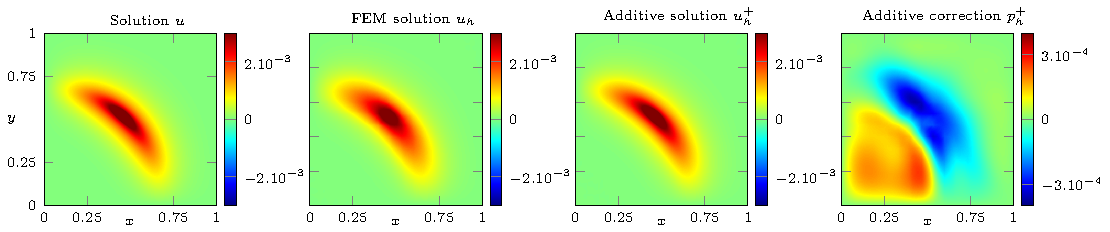
\includegraphics[width=\linewidth]{images/numeric/elliptic/plots/standalone_solutions.pdf}
		
		\vspace{8pt}
		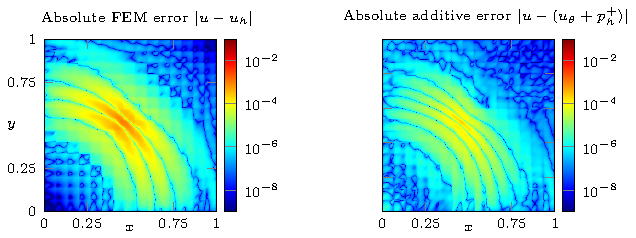
\includegraphics[width=0.7\linewidth]{images/numeric/elliptic/plots/standalone_errors.pdf}
	\end{figure}

	\vspace{-8pt}
	$$\bm{\mu}^{(2)}=(0.46,0.52,0.05,0.12)$$
\end{frame}

\subsection{2D Poisson problem on Annulus - Mixed BC}

\begin{frame}{Problem considered} 
	\textbf{Problem statement:} Considering the Poisson problem with mixed BC:
	\vspace{-5pt}
	\begin{equation*}
		\left\{
		\begin{aligned}
			-\Delta u & = f, \; &  & \text{in } \; \Omega \times \mathcal{M}, \\
			u         & = g, \;  &  & \text{on } \; \Gamma_E \times \mathcal{M}, \\
			\smash{\frac{\partial u}{\partial n}}+u  & = g_R, \;  &  & \text{on } \; \Gamma_I \times \mathcal{M},
		\end{aligned}
		\right.
		% \label{eq:Lap2DMixed}\tag{$\mathcal{P}$}
	\end{equation*}

	with $\Omega=\{(x,y)\in\mathbb{R}^2, \; 0.25\le x^2+y^2\le 1\}$ and $\mathcal{M}=[2.4,2.6]$ ($p=1$).
		
	\vspace{8pt}
	\textbf{Analytical solution :}

	\vspace{-12pt}
	\begin{equation*}
		% \label{eq:analytical_solution_Lap2D}
		u(\bm{x};\bm{\mu})= 1 - \frac{\ln\big(\mu_1\sqrt{x^2+y^2}\big)}{\ln(4)},
	\end{equation*}
	\vspace{-5pt}
	
	\textbf{Boundary conditions :}
	\begin{equation*}
		g(\bm{x};\bm{\mu})=1 - \frac{\ln(\mu_1)}{\ln(4)} \quad \text{and} \quad g_R(\bm{x};\bm{\mu})=2 + \frac{4-\ln(\mu_1)}{\ln(4)}.
	\end{equation*}

	\vspace{2pt}
	\textbf{PINN training:} MLP of 5 layers; LBFGs optimizer (4000 epochs). \\
	Imposing the mixed BC exactly in the PINN\footcite{Sukumar_2022}.

	\vspace{8pt}
\end{frame}

% \begin{frame}{Numerical results}
% 	\hspace{-5pt}\begin{minipage}[t]{0.46\linewidth}
% 		\textbf{Error estimates :} 1 set of parameters.
% 		$$\bm{\mu}^{(1)}=2.51$$
% 		\vspace{-35pt}
% 		\begin{figure}[H]
% 			\cvgFEMCorrAlldeg{images/numeric/poisson/mixed/cvg/FEM_case5_v2_param1.csv}{images/numeric/poisson/mixed/cvg/Corr_case5_v2_param1.csv}{1e-10}
% 		\end{figure}
% 	\end{minipage} \qquad \small
% 	\begin{minipage}[t]{0.48\linewidth}
% 	\end{minipage}
% \end{frame}

% \begin{frame}[noframenumbering]{Numerical results}
\begin{frame}{Numerical results}
	\hspace{-5pt}\begin{minipage}[t]{0.46\linewidth}
		\textbf{Error estimates :} 1 set of parameters.
		$$\bm{\mu}^{(1)}=2.51$$
		\vspace{-35pt}
		\begin{figure}[H]
			\cvgFEMCorrAlldeg{images/numeric/poisson/mixed/cvg/FEM_case5_v2_param1.csv}{images/numeric/poisson/mixed/cvg/Corr_case5_v2_param1.csv}{1e-10}
		\end{figure}
	\end{minipage} \qquad \small
	\begin{minipage}[t]{0.48\linewidth}
		\textbf{Gains achieved :} $n_p=50$ sets of parameters.
		$$\mathcal{S}=\left\{\bm{\mu}^{(1)},\dots,\bm{\mu}^{(n_p)}\right\}$$
		\vspace{-15pt}
		\begin{table}[H]
			\gainstableallq{images/numeric/poisson/mixed/gains/Tab_stats_case5_v2.csv}
		\end{table}

		\normalsize\centering\vspace{-20pt}
		$$h=1.33\cdot 10^{-1}$$

		\vspace{-5pt}
		Gain : $\| u-u_h\|_{L^2} / \| u-u_h^+\|_{L^2}$ \\
		\end{minipage}
\end{frame}

\begin{frame}{Numerical results}
	\begin{figure}[!ht] \centering
		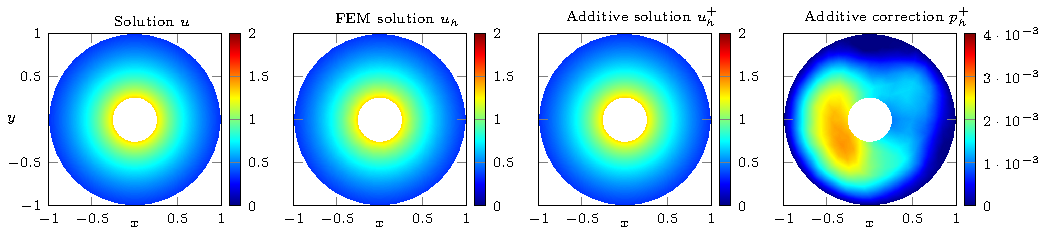
\includegraphics[width=\linewidth]{images/numeric/poisson/mixed/plots/standalone_solutions.pdf}
		
		\vspace{8pt}
		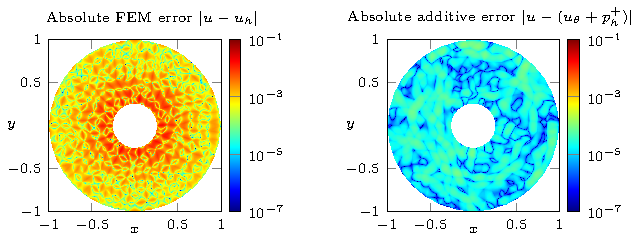
\includegraphics[width=0.7\linewidth]{images/numeric/poisson/mixed/plots/standalone_errors.pdf}
	\end{figure}

	\vspace{-8pt}
	$$\bm{\mu}^{(1)}=2.51 $$
\end{frame}

	\section{Conclusion}
	\begin{frame}[label={lastslide}]{Conclusion and Perspectives}
	\begin{itemize}
		\item PINNs are good candidates for the enriched approach.
		\item Numerical validation of the theoretical results.
		\item The enriched approach provides the same results as the standard FEM method, but with coarser meshes.
		$\Rightarrow$ Reduction of the computational cost.
	\end{itemize}

	\textbf{Perspectives :}

	\begin{itemize}
		\item Validate the additive approach on more complex geometry.
		\item Consider non-linear problems.
		\item Use the PINN prediction to build an optiaml mesh, wia a posteriori error estimates.
	\end{itemize}

	Add QR code with the paper + Image of the bean testcase
\end{frame}


	
	{\setbeamertemplate{footline}{} 	
		\begin{frame}{}
			\vspace{18pt}
			\normalsize
			\textbf{References}
			\small
			% \vspace{30pt}
			% \setstretch{0.2}
			% \AtNextBibliography{\small}
			\bibliography{biblio}
%			\printbibliography[heading=none]
		\end{frame}
	}
	\addtocounter{framenumber}{-1} 
	
	\appendix
	
	\section{Appendix}
	% \section{\appendixname~\theappendixframenumber~: Data vs PINNs}\labelappendixframe{frame:fem}

\begin{frame}{\appendixname~\theappendixframenumber~: Data vs PINNs}\labelappendixframe{frame:datavspinns}
	TODO
\end{frame}
\addtocounter{appendixframenumber}{1}

% \section{\appendixname~\theappendixframenumber~: Data vs PINNs}\labelappendixframe{frame:fem}

\begin{frame}{\appendixname~\theappendixframenumber~: Multiplicative approach}\labelappendixframe{frame:mult}
	TODO
\end{frame}
\addtocounter{appendixframenumber}{1}


\begin{frame}{\appendixname~\theappendixframenumber~: Non-linear problems}\labelappendixframe{frame:nonlinear}
	TODO
\end{frame}
\addtocounter{appendixframenumber}{1}
	
\end{document}
